\documentclass[11pt]{article}
\usepackage{colacl}
\usepackage{multirow}
\usepackage{graphicx}
\usepackage{helvet}  %Required
\usepackage{courier}  %Required
\usepackage{url}  %Required
\usepackage{subfigure}
\usepackage{algorithm}
\usepackage{algorithmic}
\usepackage{amsmath} 
\usepackage{xcolor}
\sloppy

\renewcommand{\algorithmicrequire}{\textbf{Input:}} 
\renewcommand{\algorithmicensure}{\textbf{Output:}}


\title{Spelling Correction Methods Evaluation}
%\author
%{Haonan Li \\
%haonanl5@student.unimelb.edu.au}



\begin{document}
\maketitle

\section{Introduction}

Spelling correction is an old NLP task.  From traditional non-neural methods \cite{Hall1980,Gadd1988‘,Brill2000An}, to neural methods  presents in recent years \cite{Han2011,Eger2016A,Silfverberg2016Data}. The performance of spelling correction methods has been better and better and relatively mature. 

In this paper, we investigate some old but really effective and impactful algorithms' performance on spelling correction task. Use a newly UrbanDictionary\footnote{A crowd-compiled dictionary of informal words and slang with over 7 million entries. http://urbandictionary.com} dataset.
The algorithm been evaluated includes Soundex, N-gram, Edit-distance and Editex.


\section{Methods}

In this section, we simply introduce the algorithms we evaluated in our paper. 

\noindent\textbf{Soundex} was developed by Odell and Russell, and patented in 1918 \cite{Hall1980ApproximateSM}. Uses codes based on the sound of each letter to translate a word into an at most 4 character's string. We call it Soundex code in this paper. Figure \ref{fig:soundex} shows the letter translation table and Algorithm \ref{al:soundex} describes the 4 steps processing.

\begin{algorithm}[h]
	\caption{Soundex}
	\label{al:soundex}
	\begin{algorithmic}[1]
		\REQUIRE One string 
		\ENSURE Soundex code of the string
		\STATE Except for first character, translate string characters according to table.
		\STATE Eliminate any adjacent repetitions of codes.
		\STATE Eliminate all occurrences of code 0.
		\STATE Return the first four characters.
	\end{algorithmic}
\end{algorithm}

\noindent\textbf{N-Gram} methods are string distance methods based on n-gram counts, where a n-gram of string $s$ is any substring of $s$ of some fixed length. This algorithm defines similarity of words by calculating n-gram distance, which was proposed by \cite{Ukkonen1992ApproximateSM} defines as:
\begin{equation}
|N_{s}|+|N_{t}|-2|N_{s}N_{t}|
\end{equation}
where $N_{s}$ is the set of n-gram in string $s$. 

\begin{figure}
	\centering
	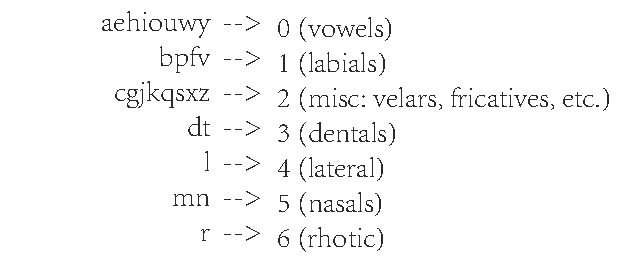
\includegraphics[width=0.5\textwidth]{img/soundex.pdf}
	\caption{Soundex letter translation table}
	\label{fig:soundex}
\end{figure}

\noindent\textbf{Edit distance} presented by \cite{Levenshtein1965Binary},  also know as Levenshtein distance, which is defined as the minimum number of elementary edit operations needed to transform one string into another. Algorithm \ref{al:editdis} gives the main part of one kind of edit distance (global edit distance) with particular distance calculation strategy.

\begin{algorithm}[htb]
	\caption{Global edit distance}
	\label{al:editdis}
	\begin{algorithmic}[1]
		\REQUIRE Two strings $s$ and $t$
		\ENSURE Edit distance between $s$ and $t$
		\STATE $ls = length(s)$, $lt = length(t)$
		\STATE Initialize $edit[0][0]=0$
		\STATE Initialize $edit[i][0]=i$, $edit[0][j]=j$
		\FOR{$i=0$ to $ls$} 
		\FOR{$j=0$ to $lt$} 
		\STATE $edit[i][j] = \min($
		\STATE $edit[i-1]j+1, $
		\STATE $edit[i][j-1]+1, $
		\STATE $edit[i-1][j-1]+equal(s[i-1],t[j-1]))$
		\ENDFOR
		\ENDFOR
		\RETURN edit[ls][lt]
	\end{algorithmic}
\end{algorithm}


\noindent\textbf{Editex} presented by \cite{Zobel1996PhoneticSM}, is a method combines phonetic matching and edit distance. In this method, alphabets also be grouped similar with Soundex, shows in Figure \ref{fig:editex} . Then, edit distance will be calculated with the grouping info, the distance between two letters in the same group defines 1 while the different groups defines 2. This scheme makes distance between similar phonetic words closer.\footnote{Because of the space limitation, we can not describe detailed algorithm, it is illustrated in our code.}

\section{Experiments}

\subsection{Data} 

\begin{figure}
	\centering
	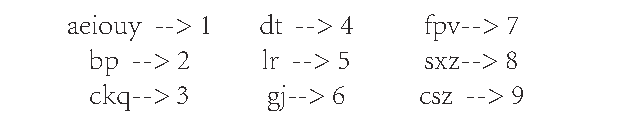
\includegraphics[width=0.5\textwidth]{img/editex.pdf}
	\caption{Editex letter groups}
	\label{fig:editex}
\end{figure}

\begin{table}
	\centering
	\begin{tabular}{c|c}
		\hline
		Item & \#Word \\
		\hline
		Testset size & 716 \\
		\hline
		Dictionary  size & 393954 \\
		\hline
		Misspelled in Dictionary & 175 \\
		\hline
		Correct not in Dictionary & 122 \\
		\hline
	\end{tabular}
	\caption{Dataset statistics (\# stands for the number of words)}
	\label{tab:dataset}
\end{table}

For our experiments we use a particular dataset:  a sub-sample of actual data posted to UrbanDictionary, in which a number of headwords taken from have been automatically identified as being misspelled \cite{Saphra2016EvaluatingIW}. This dataset simulates the spelling error data in the real world as much as possible so that is suitable for our task. Table \ref{tab:dataset} shows the statistics of our dataset.

\subsection{Setting} 

\noindent\textbf{Soundex} Calculate the Soundex code for every word and then matched with global edit distance.

\noindent\textbf{N-Gram} We evaluate the N-Gram algorithm for n in range 1 to 9. For a particular $n$, we first pad (n-1) ``$\sharp$'' in the front and end of every word. This guarantee the building of n-gram set. For example, 5-gram set for word ``he'' defined as: 
\begin{equation}
\{\sharp\sharp\sharp\sharp h, \sharp\sharp\sharp he, \sharp\sharp he\sharp, \sharp he\sharp\sharp, he\sharp\sharp\sharp, e\sharp\sharp\sharp\sharp\}
\end{equation}

\noindent\textbf{Edit Distance} There are two kinds of edit distance algorithm, local edit distance (LED) and global edit distance (GED). In this paper,  we implement both of them and evaluate them. For global edit distance, we have two distance calculation schemes : 1) (+1) for indel and mismatch and nothing to do for match; 2) (+1) for indel and mismatch and (-1) for match. The different between them will discuss in Section \ref{lab:res}. For local distance algorithm, we use (-1) for indel and mismatch and (+1) for match, and always assign 0 if 0 is better.

\noindent\textbf{Editex} We calculate the Editex follows  \cite{Zobel1996PhoneticSM} setting.
 
\section{Results \& Evaluation}\label{lab:res}

\subsection{Evaluation Method}

For all experiments in this paper, we keep all parallel best results as matched corrections for a misspelling. For example, the Soundex code for word ``adn'' is ``a35'', while for ``attain'', ``attainabilities'', ``adamas'', ``atom'' etc. are the same. No matter how many words in dictionary have the same code with ``adn'', all of them seem equally. Although this may result in a bad performance on precision when the predicted set is large.\footnote{We also do more experiments on parameter optimization. For example, randomly selecting three best matches as predicted words, which may increase precision for Soundex and local edit distance and impact recall for all algorithm. We can not list them here due to space limitation.}

\subsection{N-Gram Algorithm Evaluation}

\begin{table}
	\centering
	\small
	\begin{tabular}{c|c|c|c|c}
		\hline
		N &Predicted & Right & Precision & Recall \\
		\hline
		1 & 7150 & 183 & 2.56 & 25.56 \\
		\hline
		2 & 1484 & 151 & 10.19 & 21.09  \\
		\hline
		3 & 1429 & 149 & 10.43 & 20.81 \\
		\hline
		4 & 1426 & 148 & 10.38 & 20.67 \\
		\hline
	\end{tabular}
	\caption{N-gram algorithm results}
	\label{tab:ngram}
\end{table}

\begin{table}
	\small
	\centering
	\begin{tabular}{c|c|c|c|c}
		\hline
		Scheme &Predicted & Right & Precision & Recall \\
		\hline
		GED-1 & 5528 & 253 & 4.57 & 35.34 \\
		\hline
		GED-2 & 2497 & 204 & 8.16 & 28.49 \\
		\hline
		LED & 727774 & 133 & 0.02 & 18.58 \\
		\hline
	\end{tabular}
	\caption{Edit distance algorithm results}
	\label{tab:editdis}
\end{table}

\begin{table*}
	\centering
	\small
	\begin{tabular}{c|c|c|c|c}
		\hline
		Method &Predicted & Right & Precision & Recall \\
		\hline
		Soundex & 495146 & 436 & 0.09 & 60.89 \\
		\hline
		Local Edit Distance  & 727774 & 133 & 0.02 & 18.58 \\
		\hline
		Global Edit Distance  & 2497 & 204 & 8.16 & 28.49 \\
		\hline
		N-Gram (N=2) & 1484 & 151 & 10.18 & 21.09 \\
		\hline
		Editex & 2830 & 230 & 8.13 & 32.12 \\
		\hline
	\end{tabular}
	\caption{Full Scale results}
	\label{tab:result}
\end{table*}

We employ the original results to evaluate since the purpose of this paper is to illustrate the characteristics of different string matching algorithms through a spelling correction task, rather than find the best algorithm with parameters to correct the misspelled datasets.\footnote{The dataset we used contains only 716 words, even find the best algorithm with parameters, it might be some kind of overfitting of the particular datasets.} We use recall and precision as measured of algorithm performance follows \cite{Raghavan1989}.

The results of n-gram algorithm shows in Table \ref{tab:ngram}, in which we see that when $N=1$, the number of predicted words is large and recall is the highest. This illustrates that around 25.56\% of the misspelled words are character shifted without deletions and insertions for the best matches for $N=1$ means two words have the same consist of characters but maybe different order. However, the precision of $N=1$ is really low which makes it not a good parameter for the algorithm. $N=2$ and $N=3$ gives more balanced and significant results. For $N\geq 4$, the results are all the same. The reason might be that padding $n-1$ ``$\sharp$'' strategy for n-gram result in the related similarity tend to be stable when n is large. 


\subsection{Edit Distance Algorithm Evaluation}

Table \ref{tab:editdis} shows the results of edit distance algorithm. Which indicates that although the first two lines are both global edit distance algorithm, different distance calculate strategy leads to divergent results. Both strategies with (+1) for indels and mismatches and the difference is that first strategy do nothing for matches while the second (-1). This difference always makes the first strategy matches more result. For example, calculate the edit distance between ``aginst'' with ``against'' and ``agist''. The first strategy's result is the all equals 1 because ``against'' add one character and ``agist'' delete one character compare with ``aginst''. But the second strategy calculate -5 for ``against'' and -4 for ``agist'', which means ``against'' have more similar elements (characters) with ``against''. We could not say which one is always better in practice because it depends on the application scenarios.

As for results of local edit distance algorithm. The predicted words is explosive large but both precision and recall are not satisfactory. Which indicates that this algorithm is not suitable for the task. The reason might be that misspelled words are not tend to be a part of the corresponding corrections or reverse. Nevertheless, tt does not means local edit distance is a bad algorithm. It is very powerful in other tasks such as gene alignments \cite{Altschul1986Locally}.

\subsection{Full Scale Evaluation and Demonstration}

\begin{figure}
	\centering
	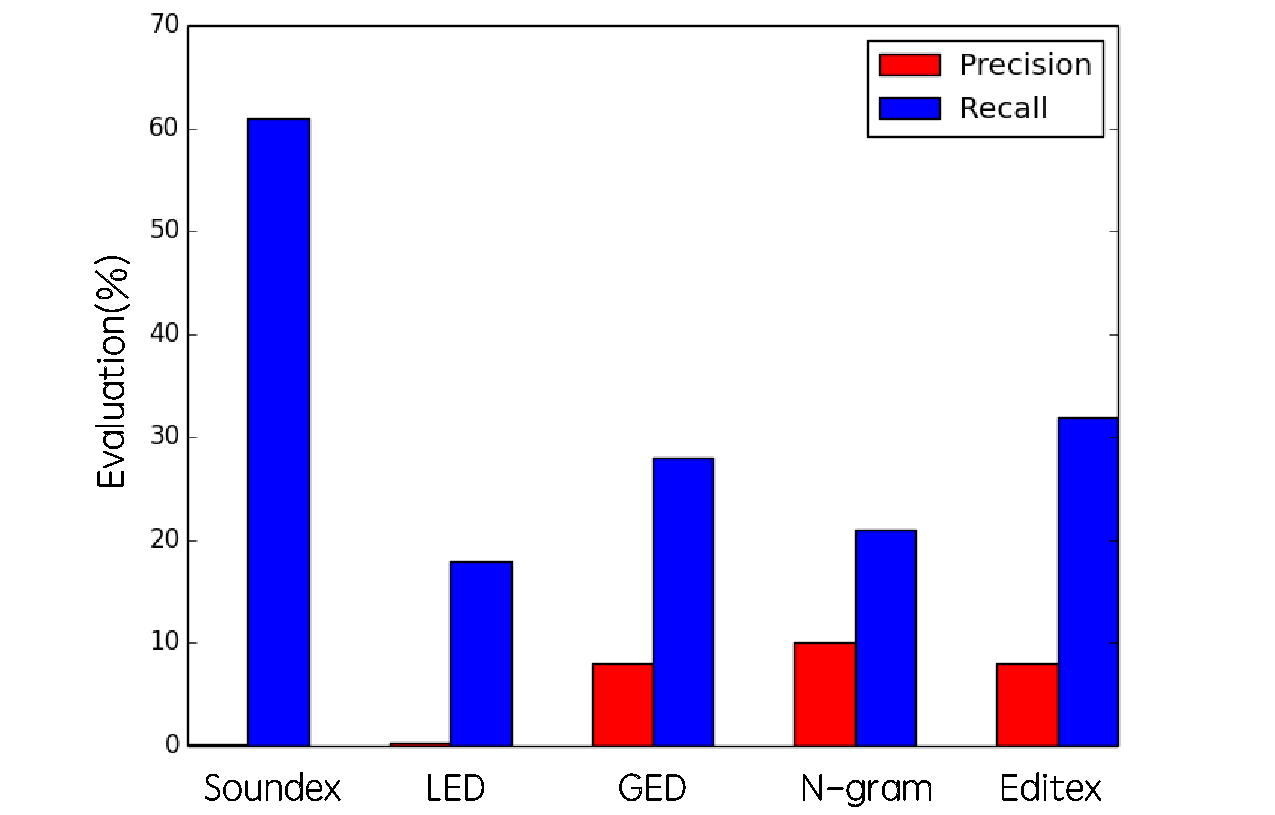
\includegraphics[width=0.5\textwidth]{img/evaluate.pdf}
	\caption{Evaluation visualization}
	\label{fig:evaluate}
\end{figure}

Table \ref{tab:result} shows a full scale evaluation and Figure \ref{fig:evaluate} is the visualization of it. Table \ref{tab:match} demonstrates output of the best match of two words for each algorithm.

Table \ref{tab:result} indicates that both Soundex and local edit distance predicted plenty of best matches. The reason for Soundex is that for words with a fixed first letter, the number of different Soundex code is only 1000 (3 digitals from 0-9). This will lead to many words have the same Soundex code. The first two lines of Table \ref{tab:match} demonstrates the Soundex's results, from which we find the pronunciation of the matched set is somewhat similar but the spelling of them various, which will leads to a number of meaningless predicts.


\begin{table*}
	\centering
	\small
	\begin{tabular}{c|c|c|c}
		\hline
		Method & Misspelled & Correct & Matched set \\
		\hline
		\multirow{2}*{Soundex} & accually & actually & akal, axile, azalea, asylees, auxiliar, ... \\
		& ahain & again & awin, annoy, aani, aoyama, anne, ayme, anay, ... \\
		\hline
		\multirow{2}*{Local Edit Distance}  & accually & actually & actually, tactually, unactually, contactually, ...  \\
		& ahain & again & disenchain, rechain, toolchain, toolchains, ... \\
		\hline
		\multirow{2}*{Global Edit Distance}  & accually & actually & actually \\
		& ahain & again & chain, amain, arain, again, ghain, alain, hain  \\
		\hline
		\multirow{2}*{N-Gram (N=2)} & accually & actually & actually, ally \\
		& ahain & again & ain  \\
		\hline
		\multirow{2}*{Editex} & actually & actually & usually, actually, annually, casually, chally, ... \\
		& ahain & again & amain,  attain, arain, again, alain, hain \\
		\hline
	\end{tabular}
	\caption{Output demonstration for all algorithms.}
	\label{tab:match}
\end{table*}

Although the precision of Soundex is extremely low,  it seems much better than local edit distance for both precision and recall, which also demonstrates in Table \ref{tab:match}.  Obviously, ``actually'' and any string with a substring  ``actually'' are treated the same. This is the trait of local edit distance, part matching.

As for global edit distance matching, it is such a pretty good algorithm for this spelling correction task that get an acceptable precision and recall. Based on the analysis of Soundex's high recall and global edit distance's high precision and recall, it is not hard to think of computing edit distance based on the Soundex results. Editex algorithm makes use of Soundex information and combine it with edit distance algorithm. 

We find that Editex gets almost the same precision with global edit distance but higher recall, which might because Editex combines the advantage of Soundex with edit distance. Form the last two rows of Table \ref{tab:match}, we find that Editex matches words with small edit distance and also considers pronunciation. 


\section{Conclusion}

We have investigated several classical approximate string matching algorithms with a particular spelling correction task and evaluated by recall and pricision. We find that Editex algorithm achieves better performance then others. Besides,  we also illustrate the characteristics of each method include n-gram, local edit distance, global edit distance with different parameters, Soundex and Editex in the paper. 


\bibliographystyle{acl}
\bibliography{bibliography}

\end{document}
